\documentclass[11pt]{article}
\usepackage{hyperref}
\usepackage[backend=biber,
  natbib=true,
  style=numeric,
  sorting=nyt]{biblatex}
\usepackage[letterpaper,margin=1in]{geometry}
\usepackage{verbatim,moreverb}
\usepackage{graphicx}
\addbibresource{defs.bib}
\addbibresource{arrpubs.bib}
\addbibresource{math.bib}
\addbibresource{tree.bib}
\begin{document}
\title{A Legofit Tutorial}
\author{Alan R. Rogers}
\date{\today}
\maketitle
\tableofcontents

\section{Introduction}
This is a tutorial on Legofit, a package that uses genetic data to
estimate the history of population size, subdivision, and admixture
\citep{Rogers:BMC-20-526, Rogers:PCJ-2-e32}. It will step you through
the process of installing the software, using it to tabulate the
frequencies of nucleotide site patterns, and then analyzing these data
to fit a model of population history. We will assume that data files
are already available in .vcf format. The full Legofit documentation
is available
\href{http://alanrogers.github.io/legofit/html/index.html}{online}.

This tutorial will be used in the 2022 edition of the AGAR
Workshop. During the workshop, we will do only last step in this
process, which estimates population history from site pattern
frequencies. We will not do the preliminary steps, which tabulate
these frequencies. Nonetheless, this tutorial describes the whole
process.

We plan to introduce students to the Center for High-Performance
Computing (CHPC) at the University of Utah, and some of the sections
below assume that you have an account on that system. (We'll be
getting accounts for everyone enrolled in the workshop.) These
sections involve using the SLURM Workload Manager to submit jobs to
the compute cluster. However, our focus during the workshop will be on
the last step, which can be done in two ways: either on the CHPC
(using SLURM), or on your own computer (using the bash shell). This
tutorial will cover both environments.

The material below is organized into the following sections:
\begin{enumerate}
\item[\ref{sec.install}] Installing Legofit on your own machine
\item[\ref{sec.chpc}] Setting up your environment at the CHPC  
\item[\ref{sec.raf}] Making an input file in .raf format
\item[\ref{sec.tabulate}] Tabulating site pattern frequencies
\item[\ref{sec.fit}] Fitting models of history
\item[\ref{sec.msma}] Model selection and model averaging
\item[\ref{sec.graph}] Graphing results
\end{enumerate}
Try to install Legofit (sec.~\ref{sec.install}) on your own before the
workshop starts. We'll help with installation problems during the
workshop, but that will take less time if you've already made a start.
The workshop will not cover
secs.~\ref{sec.raf}--\ref{sec.tabulate}. Those sections are only for
reference, when you work with Legofit on your own. During the
workshop, most of our efforts will be on fitting models
(sec.~\ref{sec.fit}), but we'll spend some time at the end on model
selection, model averaging, and graphing
(secs.~\ref{sec.msma}--\ref{sec.graph}).

\section{Installing Legofit}
\label{sec.install}
This section explains how to get Legofit running on your own
computer. It's already installed on the CHPC, so these steps are not
 needed there.
\subsection{Install git if necessary}
You may have git already. To find out whether you do, type:
\begin{verbatim}
type git
\end{verbatim}
On Mac or Linux, this will print the location of the executable git
file. If there is no such file, you'll get an error message saying
\texttt{type: git: not found}. I recommend using
\href{https://brew.sh}{homebrew} to install packages on a Mac. To
install git using homebrew, type:
\begin{verbatim}
brew install git
\end{verbatim}
Otherwise, visit \href{https://git-scm.com}{git's website} and look
for the download instructions.

\subsection{Clone legofit}
Use git to clone Legofit onto your machine. This step will create a
subdirectory called ``legofit,'' which will contain the source
code. Before executing the command below, use the \texttt{cd} command
to move into the directory where you keep source code that other
people have written. I keep such code in a directory called
\texttt{distrib}, which I originally created by typing \texttt{mkdir
  distrib}. Having created such a directory, move into it by typing
\begin{verbatim}
cd distrib
\end{verbatim}
Then clone legofit by typing:
\begin{verbatim}
git clone https://github.com/alanrogers/legofit.git legofit
\end{verbatim}
This will create a directory called legofit. Use \texttt{cd} to move into it.

\subsection{Install a C compiler if necessary}
To see whether you have a C compiler already, type \texttt{type cc},
or \texttt{type gcc}, or \texttt{type clang}. You should get output like
\begin{verbatim}
cc is /usr/bin/cc
\end{verbatim}
If you need to install a C compiler, there are several
alternatives. On a Mac, you can install Xcode from the App Store. Or
you can use Homebrew to install clang or gcc:
\begin{verbatim}
brew install clang
\end{verbatim}
or
\begin{verbatim}
brew install gcc
\end{verbatim}
On Linux, the command would be
\begin{verbatim}
sudo apt-get install clang
\end{verbatim}
or
\begin{verbatim}
sudo apt-get install gcc
\end{verbatim}

\subsection{Install ``make'' if necessary}
You will also need the program ``make,'' so type ``type make.'' If you
need to install, then
\begin{verbatim}
brew install make
\end{verbatim}

\subsection{Set up a ``bin'' directory to hold executable files.}
On Unix-like operating systems (MacOS and Linux) it is conventional
for each user to maintain a directory named ``bin,'' just below the
home directory, which contains executable files. This directory must
also be added to the system's PATH variable, which is used for finding
executable files.

First create a ``bin'' directory, if you don't already have one. To do
so, first type the command
\begin{verbatim}
cd
\end{verbatim}
at the shell prompt. This moves you into your home directory. Then
type
\begin{verbatim}
mkdir bin
\end{verbatim}
This creates a new directory called ``bin.''

You now need to add this to your shell's PATH variable. I'll assume
you're using the bash shell. In your home directory, look for a file
called either ``\verb|.bash_profile|'' or
``\texttt{.profile}''. Because the name begins with ``.'', it will not
show up if you type \texttt{ls}. However, it will appear if you type
\verb|ls .bash_profile| or \verb|ls .profile|. If only one of these
files exists, open it with a text editor (not a word processor). If
they both exist, edit ``\verb|.bash_profile|''. If neither exists, use
the editor to create a new file called ``\verb|.bash_profile|''.

Within this file, you may find existing definitions of the PATH
variable. Add the following after the last line that changes this
variable:
\begin{verbatim}
export PATH=$HOME/bin:$PATH
\end{verbatim}
Save this change and exit the editor.

The contents of this file are executed by the shell each time you log
into your computer. Since you have just created the file, your PATH
has not yet been reset. Log out and then log back in again, and your
PATH should be set. To check it, type
\begin{verbatim}
echo $PATH
\end{verbatim}
This will print your PATH.

\subsection{Compile and install legofit}
The details are in the
\href{http://alanrogers.github.io/legofit/html/index.html}{Legofit
  documentation}.

\section{Setting up your environment at the CHPC}
\label{sec.chpc}
These instructions are needed only if you're using the facilities of
the Center for High Performance Computing (CHPC) at the University of
Utah. We are in the process of getting that set up for the
workshop. The current instructions may need to change once we get that
set up.

Utah's CHPC has several ``clusters,'' each with many ``nodes.''  Each
node is a powerful computer in its own right. The
\href{https://slurm.schedmd.com/documentation.html}{SLURM} version of
the pipeline submits legofit jobs to multiple nodes so that they can
run in parallel. Within each node, legofit parallelizes across all
available cores. This greatly reduces the time required for an
analysis.

To log into a CHPC cluster, your own computer must support ssh. To
find out whether it does, type the command
\begin{verbatim}
type ssh
\end{verbatim}
at the bash prompt. If ssh is on your system, the response will be
something like
\begin{verbatim}
ssh is /usr/bin/ssh
\end{verbatim}
If ssh is not on your system, the response will be
\begin{verbatim}
-bash: type: ssh: not found
\end{verbatim}
In the latter case, install \href{https://www.openssh.com}{openssh} by
typing
\begin{verbatim}
brew install openssh
\end{verbatim}

Now that you have access to ssh, you can log into one of the CHPC
clusters by typing the following at the bash prompt. Either
\begin{verbatim}
ssh -l <your unid> notchpeak.chpc.utah.edu
\end{verbatim}
or
\begin{verbatim}
ssh -l <your unid> kingspeak.chpc.utah.edu
\end{verbatim}
or
\begin{verbatim}
ssh -l <your unid> lonepeak.chpc.utah.edu
\end{verbatim}
Here, \verb|<your unid>| is your own University of Utah id. Each of
these commands will log you onto one of the clusters at Utah's CHPC.
Then if you haven't already done so, you'll then need to set up your
CHPC environment as described above in section~\ref{sec.chpc}.

In the sections that follow, I will introduce you to several
directories and files on the CHPC servers. Each one is described by
its ``path name'' relative to your own ``home directory,'' which is
represented by the symbol \verb|~|. (In scripts, this directory is
often called \verb|$HOME|.) Before these path names will work, you'll
need to define two ``soft links'' within your own home directory,
which point to group storage devices owned by the Rogers lab. After
you define these soft links, \verb|~/grp1| will refer to one of these
group storage devices and \verb|~/grp2| to the other. You can
establish these links by typing
\begin{verbatim}
ln -s /uufs/chpc.utah.edu/common/home/rogersa-group1 ~/grp1
ln -s /uufs/chpc.utah.edu/common/home/rogersa-group2 ~/grp2
\end{verbatim}
If everyone defines these soft links in the same way, then we can all
use path names of the form \verb|~/grp1/rogers/data/whatever|.

The Legofit executables are already available directory
\verb|~/grp1/bin|. To make these easily available, use a text editor
to edit the file \verb|.bash_profile| in your home directory. Within
that file, you will find a line that defines a variable called
\texttt{PATH}, which is used by bash to find executable programs. We
want to add \verb|~/grp1/bin| to the end of \texttt{PATH}, so that
bash can find the Legofit executables. Edit that line that defines
\texttt{PATH} so that it looks like this
\begin{verbatim}
export PATH=$PATH:$HOME/bin:$HOME/.local/bin:$HOME/grp1/bin
\end{verbatim}
Also add the following line at the end of the file
\begin{verbatim}
module --latest load git
\end{verbatim}
This last line will give you access to the program ``git,'' which
you'll need to access the agar22 repository. After making these
changes, save the file and exit the editor. The file
\verb|.bash_profile| is normally read only once, when you first log
in. You've only just edited this file, bash doesn't yet know about the
changes you made there. To fix this, you can either type
\texttt{logout} and then \texttt{ssh} back in again, or type
\verb|. .bash_profile|, which tells bash to execute the commands in
this file.

Finally, clone the agar22 repository into your own home directory on
the CHPC.
\begin{verbatim}
git clone https://github.com/alanrogers/agar22.git agar22
\end{verbatim}
This will create a subdirectory called ``agar22,'' which contains
files related to the workshop.

\section{Making an input file in .raf format}
\label{sec.raf}
Legofit uses data in ``.raf'' format. The following data sets are
already available on the server at Utah's CHPC.
\begin{description}
\item[Altai Neanderthal]
\verb|~/grp1/rogers/data/altai/orig2/altai.raf.gz|

\item[Vindija Neanderthal]
\verb|~/grp1/rogers/data/vindija/orig/vindija.raf.gz|

\item[Denisovan]
\verb|~/grp1/rogers/data/denisova/orig2/denisova.raf.gz|

\item[Western Europeans (SGDP)]
\verb|~/grp1/rogers/data/simons/raf/weur.raf.gz|
\end{description}
You can use any or all of these in your projects. But you'll also need
to make at least one more. To do so, copy the following
\href{https://alanrogers.github.io/agar22/legofit/weur.slr.html}{script}
into a directory of your own:
\begin{verbatim}
~/grp1/rogers/data/simons/raf/weur.slr
\end{verbatim}
Change its name (because ``weur'' stands for ``western European'') and
edit it to reflect the population or populations that you want to
study. It's set up to run on the ``notchpeak'' cluster, where I have
only one node.

If that node is free, you can run it there by using ``cd'' to move to
the directory that contains the script and then typing
\begin{verbatim}
sbatch <your script name>
\end{verbatim}
where \verb|<your script name>| is the name of your version of the
script. This script will take many hours to complete. You can check on
its status at any time by typing
\begin{verbatim}
squeue -u <your user id>
\end{verbatim}
where \verb|<your user id>| is the id you use to log onto the CHPC cluster.
As a shorthand, I often type this as
\begin{verbatim}
squeue -u `whoami`
\end{verbatim}
which uses Linux's ``whoami'' command to fill in your user id.

If the notchpeak node is busy, try kingspeak instead. I have six nodes
there, so your odds are better. Before doing so, edit your slurm
script. The lines that read
\begin{verbatim}
#SBATCH --account=rogersa-np
#SBATCH --partition=rogersa-np
\end{verbatim}
work on notchpeak but not on kingspeak. For kingspeak, they should read
\begin{verbatim}
#SBATCH --account=rogersa-kp
#SBATCH --partition=rogersa-kp
\end{verbatim}

\section{Tabulating site patterns}
\label{sec.tabulate}
Legofit works with the frequencies of ``nucleotide site patterns,''
which are explained in 
\href{http://alanrogers.github.io/legofit/html/index.html#sitepattern}{this
  section} of the Legofit website. During the workshop, you will not
need to tabulate site patterns, because I'll do that for you before
the workshop begins. This section is here to help you do the job on
your own, after the workshop.

The Legofit package includes several programs for tabulating site
patterns. I'll focus here on ``sitepat,'' which works with data files
rather than with the output of a simulation program. Sitepat reads a
series of files in
\href{http://alanrogers.github.io/legofit/html/index.html#sitepattern}{.raf
  format} and writes a file describing the frequency of each site
pattern. Optionally, it also writes a series of output files, each
describing site pattern frequencies in a different
\href{https://en.wikipedia.org/wiki/Bootstrapping_(statistics)}{bootstrap
  replicate}. These replicates are used for measuring statistical
uncertainty. Details are in the
\href{https://alanrogers.github.io/legofit/html/sitepat.html}{Legofit
  docs}. Sitepat reads enormous data files and can take hours to run,
even on a compute cluster. That is why we aren't doing this step
during the workshop.

Have a look at file
\href{https://github.com/alanrogers/agar22/blob/main/legofit/europe/data.opf}{data.opf}. After
the header, the first few lines look like
\begin{verbatim}
#       SitePat             E[count]           loBnd           hiBnd
              x       312922.8110121  311974.2398439  313732.1909228
              y       306301.1413693  305178.5610866  307121.6833708
              v       102039.5699405  101293.0904018  102887.7097098
              a        78653.9538690   77779.2808408   79467.4795387
              d       339489.6889881  337728.6566221  341531.9807664
            x:y       189532.2514885  187871.4715776  191321.2242190
\end{verbatim}
The left column lists the site patterns. ``E[count]'' is (more or
less) the number of sites exhibiting each site pattern. (For a full
explanation, see the
\href{https://alanrogers.github.io/legofit/html/index.html#sitepattern}{Legofit
  docs}.) The values under ``loBnd'' and ``hiBnd'' enclose a 95\%
confidence interval. The frequency of site pattern ``x'' is its value
of ``E[count]'' divided by the sum of all the values under ``E[count].''

It's best to run sitepat within a script, both because it takes awhile
to run, and also because the script will document what you did.
\href{https://github.com/alanrogers/agar22/blob/main/legofit/europe/sitepat.slr}{Here}
is the slurm script that generated the output above.

\section{Fitting models of history}
\label{sec.fit}
\subsection{Organizing the data directory}
For each set of site pattern data, I create a directory tree with the
same format, which is illustrated in the github repository at
\href{https://github.com/alanrogers/agar22/tree/main/legofit/europe}{legofit/europe}. Within
this directory, you'll find (1)~a README.md file, which describes all
the others, (2)~a file called ``data.opf,'' which contains observed
site pattern frequencies, (3)~\href{sitepat.slr.html}{sitepat.slr}, a
slurm script that runs ``sitepat'' and generates ``data.opf,'' and
``boot,'' a directory containing bootstrap replicates.  There will
eventually be other files with names like ``all.bootci'' and
``all.bma,'' which contain the results of analyses.  Within this
directory, you will also find subdirectories with names like ``a,''
``ab,'' and so on. Each of these refers to a different model of
history, which we wish to fit to the data in ``data.opf.''  Name these
as you wish, but it's a good idea to keep the names short. In my
naming scheme, directory ``a'' contains a model in which there is only
one episode of admixture, labeled $\alpha$; ``ab'' is for a model that
has episodes $\alpha$ and $\beta$; and so on.

\subsection{Preliminary exercises with legosim and legofit}
Within the subdirectory for each model, assumptions about population
history are described in file ``a.lgo.''  These assumptions are
described using syntax that you can read about
\href{http://alanrogers.github.io/legofit/html/index.html#lgo}{here}.
Use \texttt{cd} to move into directory ``a,'' and have a look at
\href{https://github.com/alanrogers/agar22/tree/main/legofit/europe/a/a.lgo}{a.lgo}. Then
type this at the bash command line:
\begin{verbatim}
legosim a.lgo
\end{verbatim}
This runs the program ``legosim,'' which reads file
\href{https://github.com/alanrogers/agar22/tree/main/legofit/europe/a/a.lgo}{a.lgo},
estimates the probability of each site pattern, and prints out the
result. By default, legosim doesn't calculate probabilities for
singleton site patterns (those in which the derived allele is present
only once), and it uses a stochastic algorithm to estimate
probabilities. To include singleton site patterns and use the (faster
and more accurate)
\href{https://peercommunityjournal.org/articles/10.24072/pcjournal.132}{deterministic
  algorithm}, the command would be
\begin{verbatim}
legosim -1 -d 0 a.lgo
\end{verbatim}
Because it is fast, the legosim program is a useful way to check for
errors in your .lgo file. For further details about the program and
its command-line arguments, see
\href{http://alanrogers.github.io/legofit/html/legosim.html}{its
  documentation}.

Having ascertained that the sotware can read ``a.lgo'' without errors,
let's use the ``legofit'' program to estimate parameters. The
parameters to be estimated are those defined as ``free'' in file
``a.lgo.'' Type the following at the bash command line:
\begin{verbatim}
legofit -1 -d 0 --tol 1e-3 a.lgo ../data.opf
\end{verbatim}
After a few seconds, legofit should print a page of output. But before
examining that, let's unpack the command that generated it. The 1st
argument on the command line is ``\texttt{-1}.'' This tells legofit to
use singleton site patterns---those in which the derived allele is
present only once. Next, the arguments ``\texttt{-d 0}'' tells legofit
to use its deterministic algorithm, which is faster and more accurate
than the stochastic one it uses by default. (The stochastic algorithm
is needed for complex models.) The arguments ``\texttt{--tol 1e-3}''
tell legofit to be satisfied with a fairly loose fit between model and
data. In research, you would want a smaller number here. The next
argument, \texttt{a.lgo}, is the file describing the model of history,
and the final argument, \texttt{../data.opf}, is the data file.

Now lets examine the output of that last command. The first section of output
echoes the the legofit command and the input parameters, along with
default values of parameters that we didn't set on the command line.
\begin{verbatim}
########################################
# legofit: estimate population history #
#      version 2.3.8-12-gf1f00c9       #
########################################
#
# Program was compiled: Jun 21 2022 11:28:40
# Program was run: Thu Jul  7 20:38:55 2022
#
# cmd: legofit -1 -d 0 --tol 1e-3 a.lgo ../data.opf
# curr dir: /Users/rogers/txt/agar22/legofit/europe/a
# Stage nOptItr nSimReps
#     0    1000        1
# algorithm          : deterministic
# ignoring probs <=  : 0
# Branch length floor: 0
# DE strategy        : 2
#    F               : 0.3
#    CR              : 0.8
#    tolerance       : 0.001
# nthreads           : 2
# lgo input file     : a.lgo
# site pat input file: ../data.opf
# free parameters    : 12
# points in DE swarm : 120
# Including singleton site patterns.
# cost function      : KL
\end{verbatim}
In the output above, ``tolerance'' is the value we specified as
\texttt{--tol 1e-3} on the command line.  The next section prints the
initial values of all parameters, as read from the .lgo file.
\begin{verbatim}
Initial parameter values
Fixed:
      zero = 0
       one = 1
       TmN = 1
     Txynd = 25920
Free:
       Tnd = 24000
       Tav = 14000
       Txy = 10000
        Td = 2500
        Ta = 4000
        Tv = 1000
    twoNav = 2000
     twoNn = 2000
    twoNnd = 2000
    twoNxy = 20000
  twoNxynd = 20000
        mN = 0.01
\end{verbatim}
Then comes a line that tells us the result of the optimization procedure.
\begin{verbatim}
DiffEv reached_goal. cost=7.22802e-04 spread=8.77863e-04
\end{verbatim}
To understand this line, you need to know how legofit fits parameters
to data. It uses something called ``KL divergence''
\citep{Kullback:AMS-22-79} to measure the difference between observed
site pattern frequencies and those predicted by the model of history.
Legofit searches for parameter values that minimize KL divergence,
which is called ``cost'' in the output above. The value printed there
(7.22802e-04) is the lowest KL divergence legofit was able to
find. This search is conducted by an algorithm called ``differential
evolution'' (DE) \citep{Price:DE-06}. DE maintains a swarm of points,
each representing a guess about parameter values.  In each iteration
of the algorithm, the best points (those with lowest KL) mutate,
recombine, and reproduce to produce a new generation of points. The
algorithm stops when the difference between the best point and the
worst (called ``spread'' in the output above) falls to a specified
tolerance. As you can see in this output, spread is smaller than
0.001, the tolerance we specified using ``\texttt{--tol 1e-3}'' on the
command line. Thus, the algorithm has reached its goal, and this is
why it printed \verb|DiffEv reached_goal| in the output above. This
goal is arbitrary, and the output can be useful even when the goal is
not reached.

The next section of output lists the fitted values of all parameters.
\begin{verbatim}
Fitted parameter values
Free:
       Tnd = 24871.7
       Tav = 16727.1
       Txy = 13090.4
        Td = 1494.04
        Ta = 5346.73
        Tv = 2660.19
    twoNav = 14309.4
     twoNn = 8788.21
    twoNnd = 2998.19
    twoNxy = 23935.7
  twoNxynd = 46699.2
        mN = 0.0198353
\end{verbatim}
Finally, legofit prints the expected branch length associated with
each site pattern in the fitted model.
\begin{verbatim}
#       SitePat  BranchLen
              x 38204.0073508
              y 37200.1770458
              v 12628.3146863
              a 10003.0899715
              d 41976.1547361
            x:y 22591.0958761
            x:v 274.3861485
            x:a 278.8300856
            x:d 3121.4558596
            y:v 383.1800171
            y:a 321.8630482
            y:d 2936.3292837
            v:a 28571.5881777
            v:d 1060.8437350
            a:d 1067.6185093
          x:y:v 576.2188433
          x:y:a 571.7749063
          x:y:d 7001.3957667
          x:v:a 2884.5519560
          x:v:d 225.8439349
          x:a:d 230.2878720
          y:v:a 3460.0030731
          y:v:d 235.9020933
          y:a:d 229.1273190
          v:a:d 17599.3335385
        x:y:v:a 7238.2996703
        x:y:v:d 624.7610570
        x:y:a:d 620.3171199
        x:v:a:d 5567.0327885
        y:v:a:d 6019.8141157
\end{verbatim}
For example, the expected branch length of site pattern $x$ is
38204.0073508 generations. This is the average length, within the gene
genealogy, of the branch that, should a mutation strike it, would
generate site pattern $x$. Under the model of infinite sites
\citep{Kimura:InfiniteSites}, the expected frequency of a site pattern
among polymorphic sites is proportional to its expected length and can
be calculated as the ratio of this length to the sum of all the
lengths.

\subsection{A legofit pipeline}
\label{sec.pipeline}
A minimal legofit analysis would consist of just one run of the
program, such as the one we did above. This provides a point estimate
of each parameter but does not estimate the uncertainties of those
estimates. To estimate uncertainties, you also need to run legofit on
each bootstrap estimate. Having done all that, you have completed what
I like to call ``stage~1'' of a complete analysis.

The second stage of analysis is designed to guard against a problem
that often arises when one tries to find the minimum of a complex
function. The cost function may have many
\href{https://en.wikipedia.org/wiki/Maxima_and_minima}{local minima}
(low spots), some of which are deeper than others. We are looking for
the ``global minimum,'' which is the deepest of these local
minima. The DE algorithm is pretty good at finding global minima, but
it isn't perfect. It's possible that the legofit runs from stage~1
ended up at several local minima. Stage~2 is designed to choose among
these local minima.

To make this possible, each job in stage~1 uses the
\texttt{--stateOut} option, which tells legofit to write a file
summarizing the final state of the DE swarm. Then, each job in
stage~2 uses the \texttt{--stateIn} option, which tells legofit to
initialize its swarm of DE points by reading all the state files
produced by stage~1. Thus, each legofit job in stage~2 begins with a
DE swarm that includes points from all the legofit jobs of stage~1. If
the initial swarm includes points from several local minima, then
legofit can choose among these to find the global minimum.

In addition to multiple local minima, legofit also faces another
problem: a small increase in the value of one parameter may have
nearly the same effect as a small decrease in another. This problem
can be seen in Fig.~\ref{fig.pairs}, where some parameter estimates
are tightly correlated with others. These correlations make it hard
for the optimizer to zero in on optimal parameter values.

\begin{figure*}
  {\centering
    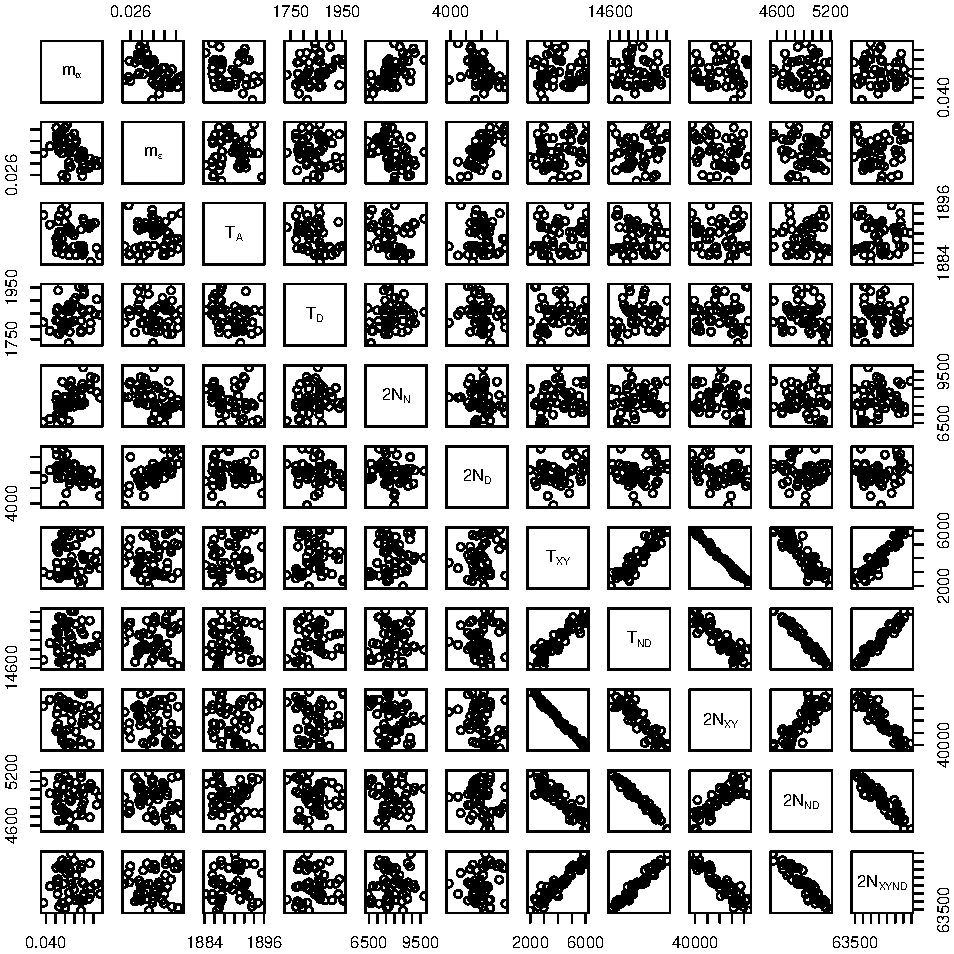
\includegraphics[width=\linewidth]{detpairs.pdf}\\}
  \caption{Scatter plot of each parameter against each other, based on
    50 simulated data sets. After \citet[Fig.~3]{Rogers:PCJ-2-e32}.}
  \label{fig.pairs}
\end{figure*}

To ameliorate this problem, I use the ``pclgo'' program (within the
Legofit package). It uses principal components analysis to reexpress
all free parameters as functions of a set of uncorrelated ``principal
components.'' Optionally, you can tell pclgo to ignore principal
components that account only for a tiny fraction of the variance. This
step rewrites a.lgo to produce a new file called ``b.lgo.'' In this
new file, all free variables are principal components, and all the
real variables are functions of the principal components.  The third
and fourth stages of analysis are just like the first and second,
except that I use b.lgo instead of a.lgo.

There are several ways to organize this four-stage analysis into a
pipeline. On the CHPC cluster, I use SLURM scripts, which are
discussed below. First, however, I will introduce a version of the
pipeline that is written entirely in bash.

\subsubsection{Bash version of pipeline}
\label{sec.bashpipe}
Within the agar22 directory tree, \texttt{cd} into directory
\texttt{legofit/europe/a}. You'll find several bash scripts there,
whose names all end with \texttt{.sh}. All but one of these scripts is
involved in the bash version of the pipeline. To experiment with this
pipeline, let's copy these scripts into a temporary directory. From
within this directory, type
\begin{verbatim}
mkdir ../tmp    # make a temporary directory
cp a.lgo ../tmp # copy .lgo file into tmp
cp *.sh ../tmp  # copy scripts into tmp
cd ../tmp       # move into that directory
rm pipeline.sh  # get rid of the file that isn't part of the bash pipeline
\end{verbatim}
Your \texttt{tmp} directory should now contain the following files:
\begin{center}
  \begin{tabular}{ll}
\texttt{a.lgo} & defines model of history\\    
\texttt{a1.sh} & stage~1 of analysis on real data\\
\texttt{a1boot.sh} & stage~1 on a bootstrap replicate\\
\texttt{a2.sh} & stage~2 on real data\\
\texttt{a2boot.sh} & stage~2 on a bootstrap replicate\\
\texttt{pclgo.sh} & run pclgo to create b.lgo  \\
\texttt{b1.sh} & stage~3 of analysis on real data\\
\texttt{b1boot.sh} & stage~3 on a bootstrap replicate\\
\texttt{b2.sh} & stage~4 on real data\\
\texttt{b2boot.sh} & stage~4 on a bootstrap replicate\\
\verb|bash_pipeline.sh| & runs all the other scripts\\
\end{tabular}
\end{center}
If you examine these scripts (for example, by typing
\texttt{less a1.sh}), you'll find that the legofit commands include
the option \texttt{-S 5000}, which tells the DE algorithm to do as
many as 5000 iterations. This could take awhile, so let's speed things
up. To change ``5000'' into ``100'' in all the files at once, type
\begin{verbatim}
sed -i "" 's/5000/100/g' *.sh 
\end{verbatim}
This will reduce the accuracy of our answers, but that's okay---this
is only an exercise. To run the first stage of analysis on the real
data, enter the following command:
\begin{verbatim}
bash a1.sh
\end{verbatim}
That command takes 2.7 seconds on my 2018 Macbook Air. After it runs,
there should be three new files in your directory:
\begin{center}
  \begin{tabular}{ll}
    a1.legofit & main output from legofit\\
    a1.err     & error output from legofit\\
    a1.state   & state of DE swarm at end of legofit run\\
  \end{tabular}
\end{center}
To run the first stage on all bootstrap replicates, type:
\begin{verbatim}
seq 0 49 | xargs -n 1 bash a1boot.sh
\end{verbatim}
This command will run 50 jobs, each of which might have been launched
by typing on the command line something like
\begin{verbatim}
bash a1boot.sh <i>
\end{verbatim}
where \verb|<i>| is 0 for the first job, 1 for the second, and so on
up to 49. Each job will analyze a single bootstrap replicate and will
write three files that are analogous to the three discussed above. It
takes several minutes to do all 50 bootstrap replicates.

We could, if we wished, proceed in this fashion and execute the
remaining stages of analysis by typing bash commands at the
terminal. But there is an easier way. Examine the file
\verb|bash_pipeline.sh| by typing 
\begin{verbatim}
less bash_pipeline.sh
\end{verbatim}
After a few lines at the top, which establish rules for dealing with
errors, you will find
\begin{verbatim}
# Stage 1 of analysis.
bash a1.sh
seq 0 49 | xargs -n 1 bash a1boot.sh
\end{verbatim}
These lines are identical to the commands we used above to execute the
first stage of analysis. The script as a whole does the entire legofit
analysis. To execute it all, you would type
\begin{verbatim}
bash bash_pipeline.sh
\end{verbatim}
You would end up with 204 .legofit files (51 for each stage), the same
number of .err files, and half that many .state files. Before talking
about what to do with these files, let us consider other ways to
implement a pipeline.

This implementation, using bash, has the advantages of simplicity and
low overhead. It's probably the easiest version to get working on your
laptop. However, there are better ways to implement a pipeline. One
problem the current approach is that when something goes wrong half
way through the analysis, it's hard to start the process up again in
the middle. Another is that we are doing only one legofit run at a
time. It would be better to do many runs in parallel.

In the bash pipeline, we used the xargs command. This has a
``\texttt{-P}'' argument, which makes it possible to run multipe jobs
in parallel. This would not be useful in the current pipeline,
however, because legofit is multithreaded and each run uses all the
cores available on your computer. To run multiple legofit jobs in
parallel, you need a compute cluster such as those available at the
University of Utah's Center for High Performance Computing (CHPC).

\subsubsection{SLURM version of pipeline}
\label{sec.slurmpipe}
Use ssh as described above to log into one of the CHPC clusters, and
then \texttt{cd} into directory
\texttt{agar22/legofit/europe/a}. You'll find several SLURM scripts
there, whose names all end with \texttt{.slr}. There is also a shell
script called ``pipeline.sh,'' which runs the entire pipeline.  To
experiment with this pipeline, let's copy these scripts into a
temporary directory. From within this directory, type
\begin{verbatim}
mkdir ../tmp          # make a temporary directory
cp a.lgo ../tmp       # copy .lgo file into tmp
cp *.slr ../tmp       # copy slurm scripts into tmp
cp pipeline.sh ../tmp # copy pipeline script
cd ../tmp             # move into that directory
\end{verbatim}
Your \texttt{tmp} directory should now contain the following files:
\begin{center}
  \begin{tabular}{ll}
\texttt{a.lgo} & defines model of history\\    
\texttt{a1.slr} & stage~1 of analysis on real data\\
\texttt{a1boot.slr} & stage~1 on a bootstrap replicate\\
\texttt{a2.slr} & stage~2 on real data\\
\texttt{a2boot.slr} & stage~2 on a bootstrap replicate\\
\texttt{pclgo.slr} & run pclgo to create b.lgo  \\
\texttt{b1.slr} & stage~3 of analysis on real data\\
\texttt{b1boot.slr} & stage~3 on a bootstrap replicate\\
\texttt{b2.slr} & stage~4 on real data\\
\texttt{b2boot.slr} & stage~4 on a bootstrap replicate\\
\verb|pipeline.sh| & runs all the SLURM scripts\\
\end{tabular}
\end{center}
To speed things up, we can reduce the number of iterations (as
explained above) by typing
\begin{verbatim}
sed -i "" 's/5000/100/g' *.slr 
\end{verbatim}
Now each legofit job will do only 100 DE iterations. The results won't
be as precise, but the pipeline will be fast. To run the first stage
of analysis on the real data, enter the following command
\begin{verbatim}
sbatch -A rogersa -p <your cluster> a1.slr
\end{verbatim}
where \verb|<your cluster>| is ``notchpeak,'' ``kingspeak,'' or
``lonepeak,'' depending on which cluster you logged into.
This queues your job for execution but does not necessarily run it
immediately. If the system is busy, it may not run for hours. To check
on the status of this job, type
\begin{verbatim}
squeue -u <your unid>
\end{verbatim}
The output will summarize the status of all jobs you've submitted to
SLURM.

To run the first stage of analysis on all bootstrap replicates, the
command is
\begin{verbatim}
sbatch -A rogersa -p <your cluster> --array=0-49 a1boot.slr
\end{verbatim}

To launch the entire pipeline, first use a text editor (e.g., vim or
emacs) to edit the file pipeline.sh. Near the top of that file, you'll
find the lines
\begin{verbatim}
export SBATCH_ACCOUNT=rogersa
export SBATCH_PARTITION=notchpeak
\end{verbatim}
Edit these lines to reflect the account and partition you are using,
then save the file and exit the editor. Finally, type
\begin{verbatim}
. pipeline.sh
\end{verbatim}
This will queue the entire pipeline for execution.

When the pipeline finishes, you'll want to copy the results back to
your own machine for analysis. One way to do this uses the
``rsync'' command, which you may need to install on your machine by
typing
\begin{verbatim}
brew install rsync
\end{verbatim}
Then, to get the results of the SLURM pipeline, type this from your
own computer:
\begin{verbatim}
rsync -Cavzbu <your_unid>@notchpeak.chpc.utah.edu:agar22/legofit/europe/tmp .
\end{verbatim}
This assumes that the results you want are on the CHPC server in a
directory called \url{~/agar22/legofit/europe/tmp}. It will create on
your own machine a directory called ``tmp'' in the directory from
which you issued the rsync command. That directory should now contain
all the results from the SLURM pipeline.

Incidentally, rsync is a fairly awkward tool for copying things back
and forth between the CHPC server and your own machine. I usually do
this by setting up a repository on github, which I can access both
from the CHPC and from my home machine. To transfer from CHPC to home,
I do \texttt{git push} from the CHPC and then \texttt{git pull} from
home. I'm not teaching you how to do this here, because this tutorial
is complicated enough already. I'm teaching the rsync approach
instead, because it's simpler.

\subsubsection{Snakemake version of the pipeline}
\label{sec.snakemake}
This section hasn't been written yet.

\section{Model selection and model averaging}
\label{sec.msma}
As discussed above, legofit uses KL divergence to measure the
difference between observed and expected site pattern frequences, and
it labels this value ``cost'' in its output. One might therefore
assume that the best model would be the one with the lowest value of
cost. This is not necessarily so, because of the problem of
\href{https://en.wikipedia.org/wiki/Overfitting}{overfitting}. Very
complex models fit not only the signal in the data, but also the
noise, and the noise in one data set does not predict that in
another. Consequently, the best-fitting model may not be the most
predictive.

To address this problem, Legofit uses the ``bootstrap estimate of
predictive error'' (bepe)
\citep{Rogers:BMC-20-526,Efron:JAS-78-316,Efron:IB-93}. This method
uses variation among data sets (the real data plus 50 replicates
generated by a moving-blocks bootstrap \citep{Liu:ELB-92-225}) to
approximate variation in repeated sampling. It fits the model to one
data set and then tests this fit against all the others. Let us apply
Legofit's ``bepe'' program to the output from the last stage of
analysis. Use \texttt{cd} to move into the directory with all your
.legofit output files, and type
\begin{verbatim}
bepe ../data.opf ../boot/boot*.opf -L b2.legofit b2boot*.legofit > b2.bepe
\end{verbatim}
On the bepe command line, we first list all the input .opf files,
beginning with the real data. Then, after \texttt{-L} we list the
corresponding .legofit output files in the same order. The first few
lines of output look like this
\begin{verbatim}
################################################
# bepe: bootstrap estimate of predictive error #
#          version 2.3.8-12-gf1f00c9           #
################################################
#
# Program was compiled: Mar 22 2022 17:40:38
# Program was run: Sat Jul  9 13:41:24 2022
# curr dir: /Users/rogers/txt/agar22/legofit/europe/tmp
#
#          bepe        DataFile     LegofitFile
1.130271806e-06        data.opf      b2.legofit
1.089578158e-06       boot0.opf b2boot0.legofit
\end{verbatim}
The first number in the left column is the bepe value of the real
data. This is the number to use in choosing among models. The numbers
below this one refer to bootstrap replicates and are use by booma,
which is discussed below.

\section{Graphing results}
\label{sec.graph}

\printbibliography

\end{document}
